\newpage
\section{The Scope of the Work}

The following sections define the roles and processes of the team developing the Cryptic Crossword Solver. 

\subsection{Organization Structure}

The project team is based largely upon democratic discussions and decisions, however to ensure that team deadlocks do not occur a project leader has been chosen. Figure ~\ref{fig:org_hierachy} reflects the hierarchy of the team.


\begin{figure}[here]
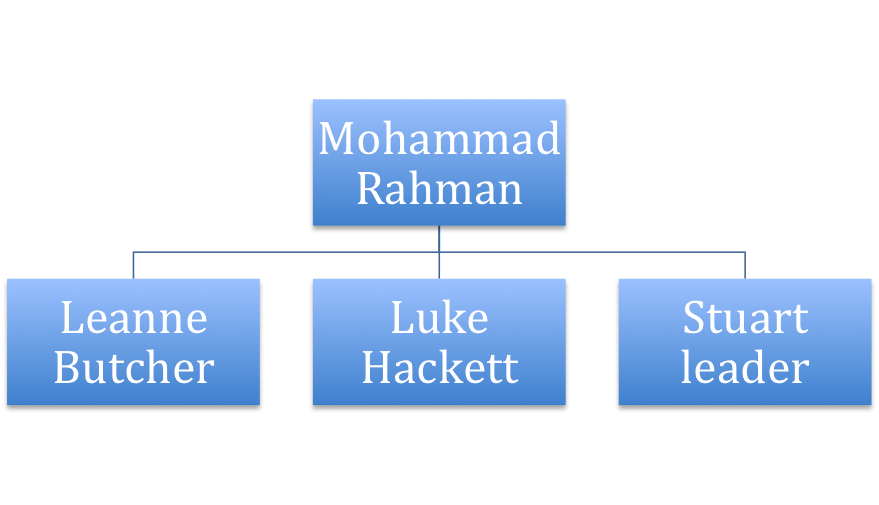
\includegraphics[width=0.9\textwidth]{requirements/functional_requirements/org_hierachy.png}
\caption{Hierarchical Structure of the team}
\label{fig:org_hierachy}
\end{figure}


\subsection{Methodology}

It has been decided that the team will follow an Agile software development model. This will allow the team to split the larger task down into smaller, more manageable ‘chunks’, that allows for a good quality analysis, evaluation, development and planning (on to the next ‘chunk’). An iterative approach is best suited for this project due to the nature of changes and updates the product will require in future builds.

This method of development also allows for a more feature-driven approach to the project. Ultimately this allows for more important features and aspects of the project to be completed first. 

Include diagram <here>


\subsection{Meetings}

A weekly meeting will take place between all project members to discuss all aspects of the project. This includes (but is not limited to) project issues, software development issues, research findings, possible improvements and code reviews.

